\section{Reconstruction and Evaluation}
\subsection{Linear images and empirical axial geometry}
We correct DNG values using per-channel black levels and white level, average the two green samples per Bayer cell, then resize by area averaging. The linear images for inversion are not JPEG-processed and do not apply any display gamma. SIFT feature matches and RANSAC similarity fits relate stationary early/late frames to the sharp reference; selected moving frames are excluded from endpoint fitting. The input and reference are separately globally normalized with the 3rd/97th-percentiles for contrast matching help. All reconstructions use the same input transform.

\Needspace{8\baselineskip}
Endpoint scales calibrate a restricted axial model. With far/near depths $z_f,z_n$, scale ratio $R$, reference depth $z_r$ and a fitted fixed pivot,
\begin{equation}
\beta(z)=\frac{z^{-1}-z_f^{-1}}{z_n^{-1}-z_f^{-1}},\qquad
s(z)=R^{\beta(z)-\beta(z_r)}.
\label{eq:scale}
\end{equation}
This interpolates log scale over inverse depth using the measured endpoints, without requiring an exact optical-origin distance from the ruler. The main dynamic warp scales about the pivot. Endpoint rotation is used for reference registration and enters the dynamic warp only in a sensitivity check. Range alone does not recover continuous target tilt or lateral drift.

\begin{figure}[t]
\centering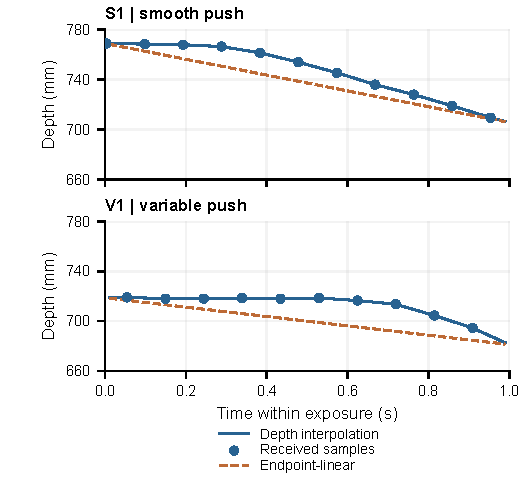
\includegraphics[width=\columnwidth]{images/trajectories.pdf}
\caption{Depth during two selected exposures. S1 and V1 contain 11 and 10 valid received samples. The models share the same exposure-boundary depths and differ only in the interior trajectory. A smooth-push instruction does not impose constant speed.}
\label{fig:depth}
\end{figure}

\Needspace{12\baselineskip}
\subsection{LiDAR-guided axial scale-blur model}
An exposure combines differently scaled views of one sharp reference-plane image $x$. We write the observation $y$ as
\begin{equation}
\begin{aligned}
y&=A(z,u)x+\epsilon,\\
A&=\sum_{k=1}^{48} w_k W[s(z_k)],\\
w_k&=\frac{0.19+0.81u_k}{\sum_j(0.19+0.81u_j)},
\end{aligned}
\label{eq:forward}
\end{equation}
Here, $z_k$ is interpolated depth, $W[s(z_k)]$ scales the image about the fitted pivot, and $u_k$ is the logged binary state after the time shift. We approximate the exposure integral with 48 midpoint bins interpolated from 10--11 received depth frames. $W$ uses sparse bilinear interpolation with replicated boundaries. The weights approximate relative irradiance, with 0.19 as the illumination floor in the black state. Each of the columns of $ A $ is the response to one point in the image - a discrete point spread function (PSF). Expansion moves points farther from the fixed scaling pivot more strongly, so the PSF varies spatially across the image. Reconstruction therefore requires inverting a spatially varying operator.

\subsection{TV-regularised reconstruction}
Once the records and endpoint geometry fix $A$, we estimate the image by non-blind, TV-regularised least squares:
\begin{equation}
\hat x=\arg\min_{0\leq x\leq1}\tfrac12\|Ax-y\|_2^2+\lambda\,\mathrm{TV}(x),
\qquad\lambda=0.002.
\label{eq:inverse}
\end{equation}
The data term fits the recorded blur, while TV limits unstable fluctuations. We use 320 outer iterations of an accelerated proximal-gradient scheme inspired by FISTA\cite{fista}, a power-estimated step size and up to 35 inner TV iterations. The TV step is approximate, and clipping constrains intensities to $[0,1]$. The comparator replaces measured $z(t)$ with constant depth velocity between the same boundary depths. Both methods share the image, light weights, geometry, solver and mask. We also evaluate the blurred input and denoise-only processing ($A=I$). Parameters are shared across trials.

\subsection{Scoring and numerical checks}
We map all 16 attempts into one canonical reference frame and fix a geometry-only intersection mask before scoring (Fig.~\ref{fig:mask}). PSNR uses unit intensity range; Gaussian-window SSIM uses $\sigma=1.5$ and population covariance\cite{ssim}. Methods receive no separate post-reconstruction alignment or contrast fit. The reference is used for registration, normalization and scoring, making this a reference-assisted experiment.

Identity, row-sum and adjoint errors are below $8\times10^{-7}$. Synthetic inversion improves PSNR from 13.99 to 27.15\,dB. Doubling the iterations from 320 to 640 changes PSNR by at most 0.049\,dB; changing the bins from 48 to 96 changes it by at most 0.207\,dB. These checks assess numerical integrity. The physical captures test how well the model describes practice.

\begin{figure}[t]
\centering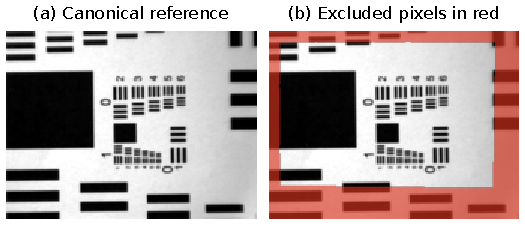
\includegraphics[width=\columnwidth]{images/evaluation_mask.pdf}
\caption{A common reference and common mask for all trials and all methods. Excluded pixels marked in red. Scores use the remaining 28327 pixels (65.6\% of the $240\times180$ image) within the irregular mask, rather than only its boundary or a rectangular display crop.}
\label{fig:mask}
\end{figure}
